% !TEX root = ../main.tex

\begin{figure}[t]
\centering
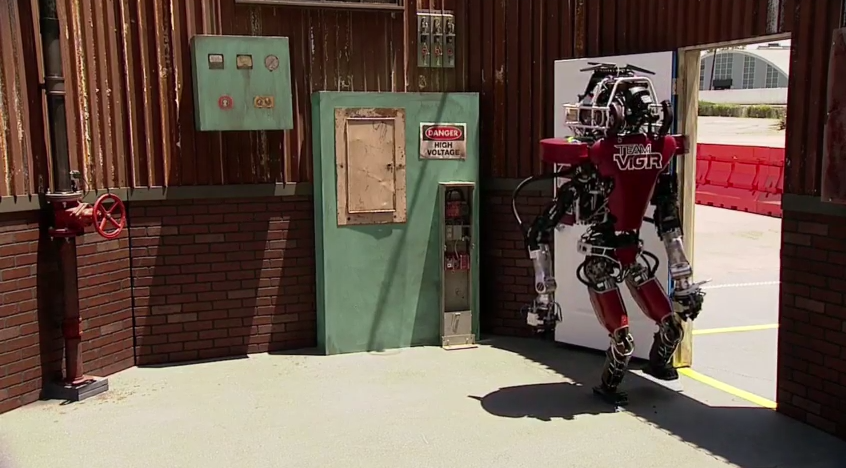
\includegraphics[width=0.99\columnwidth,clip]{./img/atlas_door_finals.png}
\caption{Team ViGIR's Atlas humanoid robot on the first day of the DRC Finals. (Photo credit: DARPA)
}
\label{Fig:AtlasDoorFinals}
\end{figure}

In preparation for the 2015 DARPA Robotics Challenge (DRC) Finals, Team ViGIR, as well as many other teams, developed an approach to high-level robot control \cite{Philipp2013Bsc, Philipp2015Msc}.
However, these approaches relied on experts developing scripted behaviors or, in the case of Team ViGIR, manually designing state machines.
In addition, there was no guarantee that the resulting high-level behavior was correct \ac{wrt} the task at hand.
Moreover, many participants observed that such approaches were fragile in practice \cite{DRC-what-happened}.

Motivated by these shortcomings, we present an approach for the automatic generation of software that implements high-level robot behaviors in a provably-correct manner.
This was enabled in part by recent advances in the field of formal methods for robotics.
Specifically, correct-by-construction mission plans can be automatically synthesized from high-level, logic-based specifications [cite ALL the papers].

\begin{myExample}\label{Ex:PickupObject}
	Consider the task, ``Walk to the valve and turn it" (Fig. \ref{Fig:AtlasDoorFinals}).
	This would be an intuitive way to express the task from a non-expert user's point-of-view.
	However, this task specification is not formal, it does not account for the robot's capabilities -- a robot with no means of locomotion or manipulation wouldn't even be able to carry it out -- and it does not specify what should happen if a failure occurs. % manipulation?
\end{myExample}

However, writing a formal, logic-based specification is a non-trivial task that requires expert knowledge.
In this paper, we automatically generate the logic-based specifications from a higher level, partial, multi-paradigm specifications: a description of the system's capabilities, the task's goals, and the task's initial conditions.
Furthermore, most approaches in this field assume that the simple, low-level components that make up the high-level plan will work as expected, i.e., they never fail.
In this paper, we take a first step towards lifting this assumption by formally accounting for the possibility of failure when executing the low-level components.
We achieve this by generalizing the concepts of ``activation" and ``completion", which were introduced in \cite{Vasu2013ICRA} to deal with the time semantics of logic-based specifications.
While a failure is still a failure and there might be no way to recover, we can still achieve \emph{graceful degradation}.

Furthermore, ours is an end-to-end approach that starts with an informal specification and results in an executable software implementation of a high-level plan.
We first create a discrete abstraction of the problem and automatically construct a formal task specification in a fragment of Linear Temporal Logic (\textsc{LTL}).
We then synthesize a \emph{reactive} mission plan that is guaranteed to satisfy the formal specification.
Finally, in an effort to bridge the gap between theoretical results and practice, we automatically generate the implementation of a state machine that instantiates the synthesized plan in software.

In this paper, we present and experimentally validate the proposed approach in the context of a Boston Dynamics Atlas humanoid robot running the software that Team ViGIR developed for the DRC (Fig. \ref{Fig:AtlasDoorFinals}).
However, the concepts apply to different systems.
We have implemented and open-sourced the proposed approach as a collection of Robot Operating System (ROS) packages \cite{ROS2009ICRA, ROS}.

\subsubsection*{Literature Survey}
Our work generalizes that in \cite{Vasu2013ICRA}, which allows us to reason about multiple outcomes of an action, such as failure, in the formal specification.
The approaches in \cite{Jon2015ICRA} and \cite{Kavraki2012ICRA} deal with the related problem of uncertainty in mobile robot motion.
In terms of our approach to creating the formal specification, some other options would have been asking the user to (i) write the formal specification, e.g., \textsc{ltl} formulas, directly, (ii) write Structured English statements \cite{JFRKG2012ICRA}, or (iii) specify the task in natural language \cite{Lignos2015AURO}.
Each option comes with trade-offs and we chose one where the user input is essentially minimal.
In terms of the mission planning step, we opted for \textsc{gr(1)}, i.e., reactive \textsc{ltl}, synthesis \cite{Bloem2012GR1} over other approaches.
These included classical AI planners, such as STRIPS \cite{STRIPS1971AI} and PDDL \cite{PDDL1998TR}, optimization under \textsc{ltl} constraints \cite{Wolff2014ICRA}, and, most notably, synthesis from co-safe \textsc{ltl} specifications, e.g., \cite{Kavraki2015ICRA}.
Our main reason for choosing \textsc{gr(1)} synthesis is the ability to specify reactivity \ac{wrt} a dynamic, and even adversarial (worst-case), environment (such as external events and component failures).
Finally, \cite{Ankur2015ISRR} also presents an end-to-end approach (from formal specification to software generation), while the toolkit presented in \cite{Finucane2010IROS} employs an executive that executes the abstract synthesized automaton.
However, in both of those cases, the user has to write a Structured English \cite{JFRKG2012ICRA} specification that exactly maps to \textsc{ltl}, a non-trivial task.

The rest of this paper is organized as follows.
In Section \ref{S:prelim}, we introduce Atlas, Team ViGIR's approach to the DRC, and Linear Temporal Logic.
In Section \ref{S:problem}, we state the problems that this paper addresses.
Sections \ref{S:abstraction} through \ref{S:synthesis} present the proposed approach, while Section \ref{S:implementation} summarizes its ROS implementation.
We present experimental demonstrations in Section \ref{S:experiments}.
Finally, we draw conclusions and propose future research directions in Section \ref{S:conclusion}.

%END